\documentclass[12pt]{article}
\usepackage{hyperref}
\usepackage{xcolor}
\usepackage{framed}
\usepackage{listings}
\usepackage{graphicx}
\usepackage{float}
\usepackage{pdfpages}
\usepackage[utf8]{inputenc}
\usepackage[T1]{fontenc}

\usepackage{titlesec}
\newcommand{\sectionbreak}{\clearpage}

\makeatletter
\renewcommand{\@seccntformat}[1]{}
\makeatother

\setlength{\parindent}{0pt}
%\newcommand{\response}[1]{{\leavevmode\color{blue}[#1]}}
\newcommand{\response}[1]{\color{blue}{#1}\color{black}}

\definecolor{mygreen}{rgb}{0,0.6,0}
\definecolor{mygray}{rgb}{0.5,0.5,0.5}
\definecolor{mymauve}{rgb}{0.58,0,0.82}
\definecolor{light-gray}{gray}{0.95}

\lstset{ %
  backgroundcolor=\color{light-gray},   % choose the background color
  basicstyle=\footnotesize,        % size of fonts used for the code
  breaklines=true,                 % automatic line breaking only at whitespace
  captionpos=b,                    % sets the caption-position to bottom
  commentstyle=\color{mygreen},    % comment style
  escapeinside={\%*}{*)},          % if you want to add LaTeX within your code
  keywordstyle=\color{blue},       % keyword style
  stringstyle=\color{mymauve},     % string literal style
}

\begin{document}

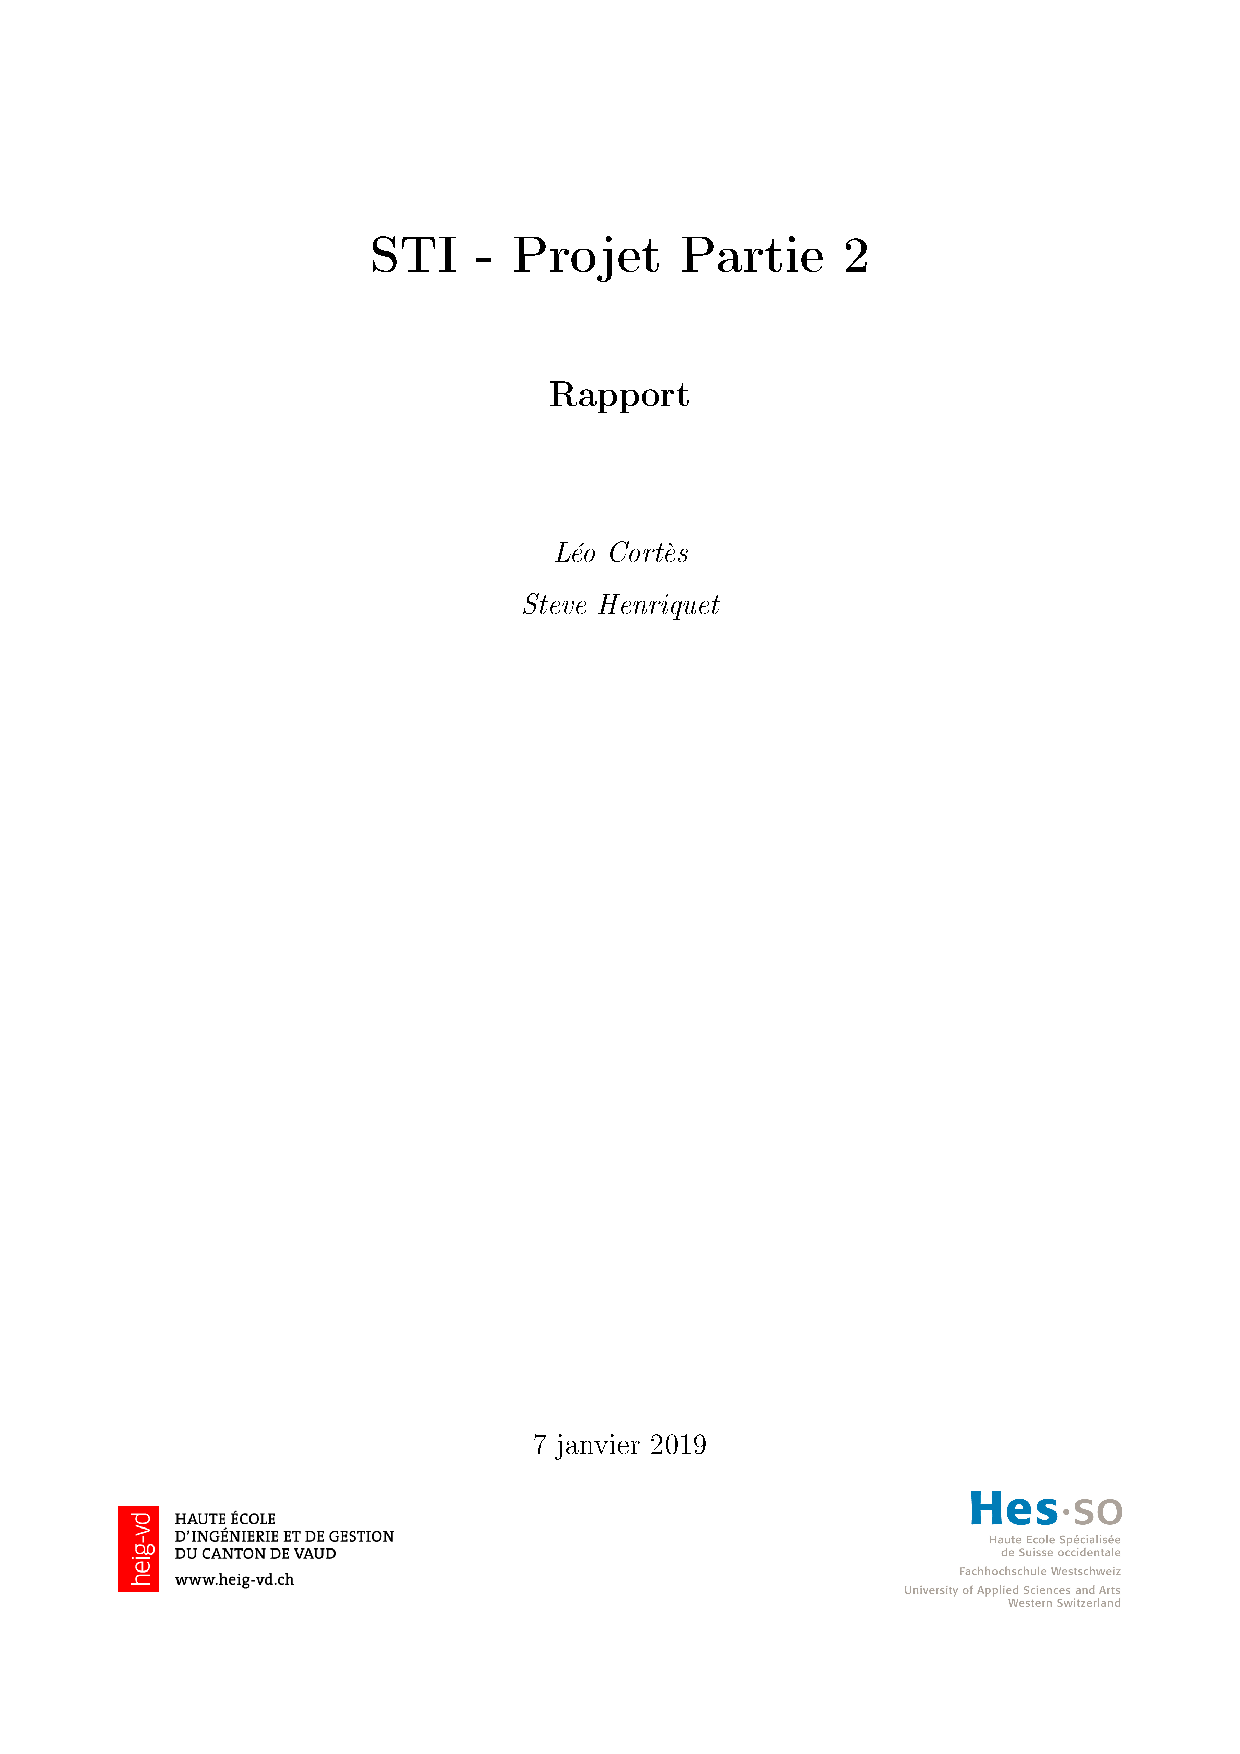
\includepdf{titre/titre.pdf}

\tableofcontents

\newpage
\section{Introduction}


\section{Vulnérabilités et corrections}
\subsection{XSS}
\subsubsection{Exploitation}
Le programme est vulnérable aux attaques XSS. Les balises HTML sont correctement inteprétée, ainsi que les balises de script. C'est problématique car un attaquand pourrait envoyer un message malicieux à un administrateur. Lorsque l'admin se connecte, le script pourrait récupérer ses cookies et l'attaquant pourrait les rejouer et devenir donc administrateur.

Voici le message envoyé par un attaquant quelconque : 
\begin{figure}[H]
\centering
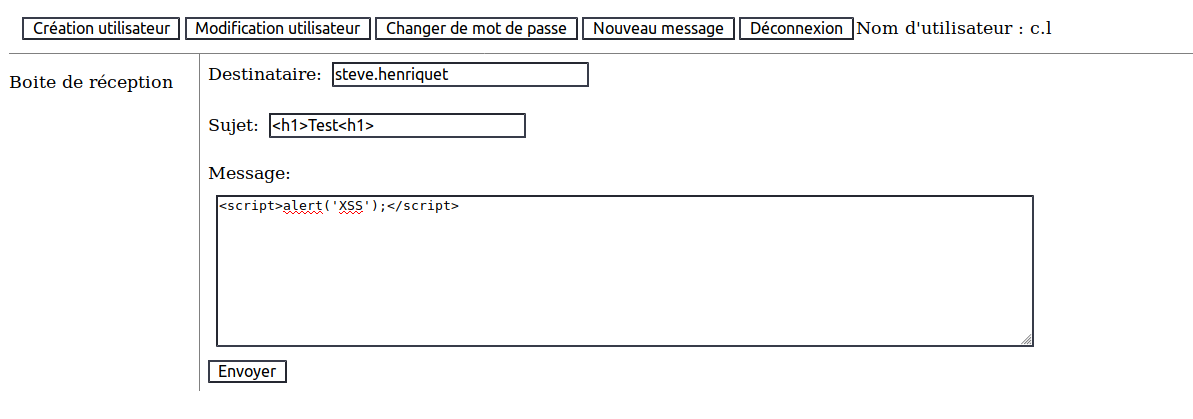
\includegraphics[width=\linewidth]{images/xssAttack.png}
\caption{Message malicieux}
\end{figure}

Voici le résultat dans la boîte de réception de la victime.
\begin{figure}[H]
\centering
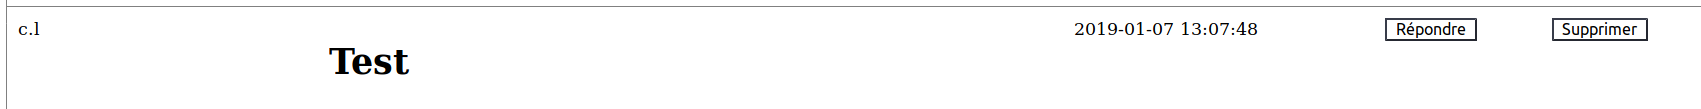
\includegraphics[width=\linewidth]{images/xssRecep.png}
\caption{Boîte de réception}
\end{figure}

Lorsque la victime l'ouvre, voici le script est correctement exécuté.
\begin{figure}[H]
\centering
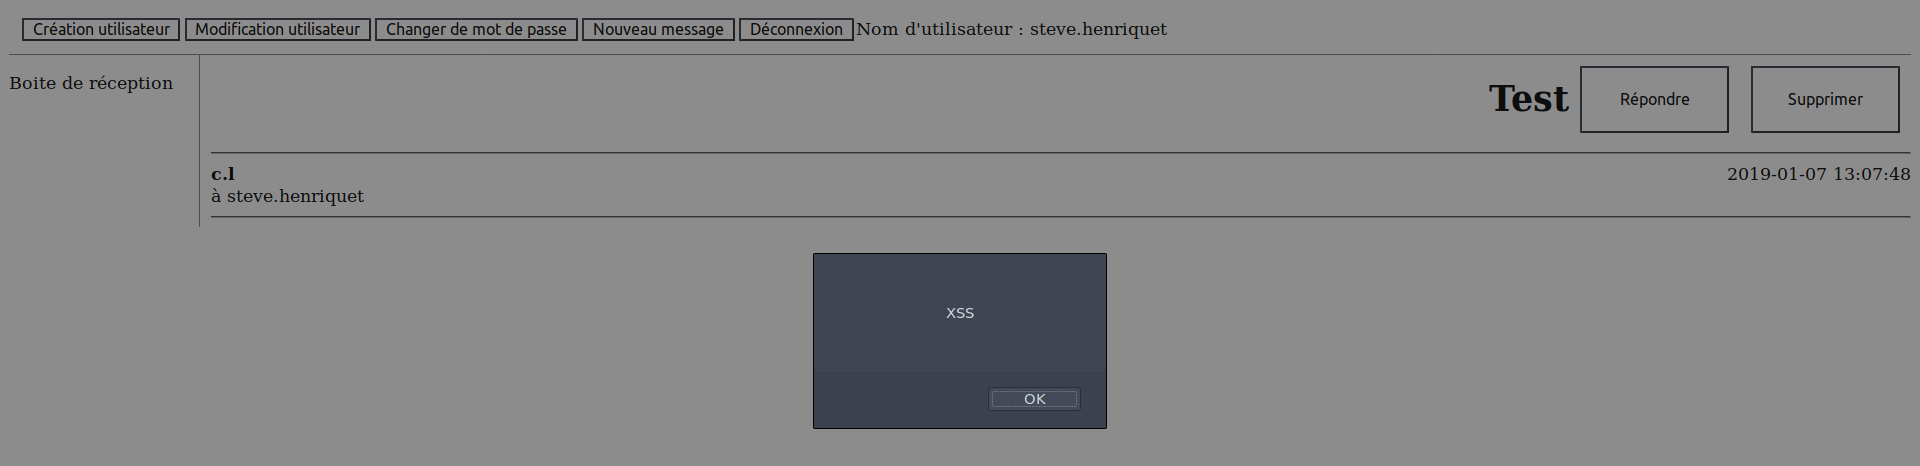
\includegraphics[width=\linewidth]{images/xssOpen.png}
\caption{Exécution XSS}
\end{figure}

\subsubsection{Correction}
Les entrées ont du être "sanitisées". Nous avons utilisé le filtre \textit{FILTER\_SANITIZE\_STRING} dans les divers inputs accessibles.
\begin{figure}[H]
\centering
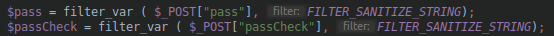
\includegraphics[width=\linewidth]{images/sanitize.png}
\caption{Exemple d'assainisation}
\end{figure}

\subsection{Injection SQL}
\subsubsection{Exploitation}
\subsubsection{Correction}
Tout comme pour les failles XSS, les entrées ont du être assainies.

\subsection{Problèmes non résolvables}
\begin{itemize}
\item PHP 5.6
\item Gestion des cookies de session
\end{itemize}

\end{document}